%% Supplementary material. Every number is a macro from tables/numbers.tex or a generated table.
\documentclass[pdflatex,sn-mathphys-num]{sn-jnl}
\usepackage{graphicx,booktabs,amsmath,amssymb,url}
% Generated by tools/research/phase7/make_tables.py from research/phase7/results. Do not edit.
\newcommand{\devParts}{151}
\newcommand{\devAllParts}{316}
\newcommand{\devNFMzero}{6.07}
\newcommand{\devNFMone}{1.25}
\newcommand{\devNegMone}{9}
\newcommand{\devWorstMone}{25}
\newcommand{\devNFMfour}{1.23}
\newcommand{\devNegMfour}{8}
\newcommand{\devWorstMfour}{11}
\newcommand{\devNFMnine}{1.29}
\newcommand{\devNegMnine}{11}
\newcommand{\devWorstMnine}{37}
\newcommand{\devNFJoint}{1.29}
\newcommand{\devNegJoint}{10}
\newcommand{\devWorstJoint}{10}
\newcommand{\devHybridNF}{1.32}
\newcommand{\devHybridWorst}{2}
\newcommand{\devRobustMzero}{80.1}
\newcommand{\devLoadMzero}{58.9}
\newcommand{\devRobustVtwoMzero}{84.1}
\newcommand{\devLoadVtwoMzero}{64.9}
\newcommand{\devRobustMone}{84.8}
\newcommand{\devLoadMone}{45.0}
\newcommand{\devRobustVtwoMone}{90.7}
\newcommand{\devLoadVtwoMone}{48.3}
\newcommand{\devRobustMfour}{85.4}
\newcommand{\devLoadMfour}{55.0}
\newcommand{\devRobustVtwoMfour}{92.7}
\newcommand{\devLoadVtwoMfour}{60.3}
\newcommand{\devRobustMnine}{88.7}
\newcommand{\devLoadMnine}{39.1}
\newcommand{\devRobustVtwoMnine}{96.0}
\newcommand{\devLoadVtwoMnine}{46.4}
\newcommand{\devRobustJoint}{89.4}
\newcommand{\devLoadJoint}{56.3}
\newcommand{\devRobustVtwoJoint}{96.7}
\newcommand{\devLoadVtwoJoint}{62.3}
\newcommand{\devJointMzeroRobust}{+9.3}
\newcommand{\devJointMzeroRobustCI}{[2.6, 15.9]}
\newcommand{\devJointMzeroLoad}{-2.6}
\newcommand{\devJointMzeroLoadCI}{[-9.3, 4.0]}
\newcommand{\devJointMoneRobust}{+4.6}
\newcommand{\devJointMoneRobustCI}{[0.0, 9.3]}
\newcommand{\devJointMoneLoad}{+11.3}
\newcommand{\devJointMoneLoadCI}{[5.3, 17.2]}
\newcommand{\devMfourMoneLoad}{+9.9}
\newcommand{\devMfourMoneLoadCI}{[4.6, 15.9]}
\newcommand{\devMnineMoneRobust}{+4.0}
\newcommand{\devMnineMoneRobustCI}{[-0.7, 8.6]}
\newcommand{\devVtwoHeld}{3423}
\newcommand{\devVtwoNotVthree}{128}
\newcommand{\devTurnOverFifteen}{3.7}
\newcommand{\devFlipLow}{18.4}
\newcommand{\devFlipMid}{7.4}
\newcommand{\devFlipHigh}{6.1}
\newcommand{\artAgreeMin}{95}
\newcommand{\artAgreeMax}{97}
\newcommand{\artKappaMin}{0.74}
\newcommand{\artKappaMax}{0.82}
\newcommand{\artKappaTwoKg}{0.60}
\newcommand{\artHeldTwoKgVthree}{57}
\newcommand{\artHeldTwoKgArt}{40}
\newcommand{\artGrasps}{430}
\newcommand{\artJointMoneLoad}{-3.3}
\newcommand{\artJointMoneLoadCI}{[-10.6, 4.0]}
\newcommand{\artJointMzeroLoad}{-17.2}
\newcommand{\artJointMzeroLoadCI}{[-24.5, -10.6]}
\newcommand{\artJointMzeroRobust}{+8.0}
\newcommand{\artJointMzeroRobustCI}{[2.0, 13.9]}
\newcommand{\artTrackMax}{0.119}
\newcommand{\repAUCLzero}{0.9958}
\newcommand{\repNFLzero}{1.316}
\newcommand{\repNFLtwo}{1.494}
\newcommand{\repNFLten}{1.425}
\newcommand{\repLtwoLzero}{1.135}
\newcommand{\repLtwoLzeroCI}{[1.035, 1.248]}
\newcommand{\repLeightLtwo}{1.014}
\newcommand{\repLeightLtwoCI}{[0.969, 1.059]}
\newcommand{\repLeightPerm}{0.999}
\newcommand{\repLeightPermCI}{[0.955, 1.042]}
\newcommand{\repLtenLtwo}{0.954}
\newcommand{\repLtenLtwoCI}{[0.907, 0.998]}
\newcommand{\repLtenPerm}{0.945}
\newcommand{\repLtenPermCI}{[0.898, 0.995]}
\newcommand{\repLsevenLtwo}{0.989}
\newcommand{\repLsevenLtwoCI}{[0.944, 1.031]}
\newcommand{\repLelevenLtwo}{1.010}
\newcommand{\repLelevenLtwoCI}{[0.961, 1.060]}
\newcommand{\repLGLtwo}{0.932}
\newcommand{\repLGLtwoCI}{[0.872, 0.991]}
\newcommand{\repLDLtwo}{0.936}
\newcommand{\repLDLtwoCI}{[0.875, 1.001]}
\newcommand{\repRankLtwo}{1.007}
\newcommand{\repRankLtwoCI}{[0.940, 1.076]}
\newcommand{\repVisibleShare}{88}
\newcommand{\fewFirstShare}{87}
\newcommand{\fewCeiling}{1.30}
\newcommand{\fewCeilingMs}{5.2}
\newcommand{\fewFixedS}{0.57}
\newcommand{\crossForty}{0.94}
\newcommand{\crossFortyCI}{[0.74, 1.19]}
\newcommand{\crossFortyViable}{79}
\newcommand{\crossHundredtwenty}{1.07}
\newcommand{\crossHundredtwentyCI}{[0.99, 1.16]}
\newcommand{\crossHundredtwentyViable}{254}
\newcommand{\powerPtwo}{0.994}

\begin{document}
\title{Supplementary material: Learning where to look first without losing robustness}
\author{\fnm{Eduardo} \sur{P\'erez Gonz\'alez}}
\affil{\orgname{Independent Researcher}, \orgaddress{\city{Zaragoza}, \country{Spain}}}
\abstract{Protocol summary, deviations, full development tables, secondary confirmatory results and sensitivity analyses. Source files: research/phase7 of the project repository.}
\maketitle

\section{Protocol, freeze and deviations}
The development protocol (part I) was committed before the development experiments; the confirmatory protocol (part II), the hypotheses, the frozen models and the test manifest were committed together (commit \texttt{de22a8a}) before any confirmatory object was planned, and signed by SHA-256 hashes in \texttt{PHASE7\_MODEL\_FREEZE.json}. Disclosed deviations: (D1) the cells of two primary objects (positions 0 and 1) were built, geometry only, during pipeline development; (D2) the H5 target became the linear-branch variant L10 and its controls were added after L10's development result; (D3) load tolerance was moved from the primary to the secondary family after the articulated development pilot; (D4) the collision decomposition settings were chosen on excluded objects (positions 500--502).

\section{Development: representation benchmark}
\begin{table}[h]
\caption{All representation variants (316 parts, out of fold; MLPs averaged over three seeds).}
\centering\scriptsize
% Generated by make_tables.py
\begin{tabular}{llrrrrr}
\toprule
Id & Model & AUC & ECE & $N_F$ & S@1 & Robust \\
\midrule
L0 & Gradient boosting, 19 features & 0.9958 & 0.0030 & 1.316 & 0.642 & 0.927 \\
L1 & Logistic regression & 0.9846 & 0.0046 & 1.890 & 0.525 & 0.947 \\
L2v & MLP, candidate only & 0.9944 & 0.0022 & 1.491 & 0.606 & 0.903 \\
L2 & MLP, + geometry $u$ & 0.9755 & 0.0194 & 1.494 & 0.599 & 0.903 \\
L3 & MLP, + DINOv2 (linear) & 0.9945 & 0.0039 & 1.422 & 0.612 & 0.879 \\
L4 & MLP, + DINOv3 (linear) & 0.9939 & 0.0043 & 1.422 & 0.611 & 0.890 \\
L5 & MLP, + DINOv2 & 0.9945 & 0.0033 & 1.417 & 0.614 & 0.912 \\
L6 & MLP, + DINOv3 & 0.9941 & 0.0035 & 1.465 & 0.599 & 0.901 \\
L7 & MLP, $u$ + DINOv2 & 0.9664 & 0.0287 & 1.478 & 0.595 & 0.901 \\
L8 & MLP, $u$ + DINOv3 & 0.9661 & 0.0291 & 1.516 & 0.580 & 0.894 \\
L9 & MLP, $u$ + untrained ViT & 0.9933 & 0.0038 & 1.472 & 0.606 & 0.883 \\
L10 & MLP, $u$ + DINOv3 (linear) & 0.9752 & 0.0205 & 1.425 & 0.611 & 0.901 \\
L10p & L10 with permuted DINOv3$^\dagger$ & 0.9919 & 0.0058 & 1.508 & 0.593 & 0.907 \\
L10r & L10 with untrained ViT$^\dagger$ & 0.9852 & 0.0120 & 1.472 & 0.602 & 0.890 \\
L8p & L8 with permuted DINOv3 & 0.9922 & 0.0048 & 1.518 & 0.595 & 0.914 \\
L11 & MLP, $u$ + OpenCLIP & 0.9657 & 0.0298 & 1.509 & 0.595 & 0.892 \\
LG & MLP, $u$ + local geometry & 0.9837 & 0.0136 & 1.392 & 0.611 & 0.846 \\
LD & MLP, $u$ + local DINOv3 & 0.9741 & 0.0228 & 1.399 & 0.612 & 0.868 \\
LGD & MLP, $u$ + both local & 0.9633 & 0.0315 & 1.441 & 0.594 & 0.896 \\
L2-rank & L2, listwise loss & 0.9887 & 0.0110 & 1.505 & 0.587 & 0.854 \\
L8-rank & L8, listwise loss & 0.9882 & 0.0099 & 1.540 & 0.577 & 0.879 \\
\bottomrule
\end{tabular}

\end{table}

\section{Development: physics corrections and sensitivity}
Under the previous criterion \devVtwoHeld{} trials were held; \devVtwoNotVthree{} of them fail the rotation-and-contact criterion. Verdict changes relative to torsion 0.005~m: \devFlipLow\% (0.001), \devFlipMid\% (0.0025), \devFlipHigh\% (0.02). Development contrasts (v3): M4$-$M1 load tolerance \devMfourMoneLoad{} \devMfourMoneLoadCI; M9$-$M1 robustness \devMnineMoneRobust{} \devMnineMoneRobustCI; Joint$-$M1 robustness \devJointMoneRobust{} \devJointMoneRobustCI. Full per-condition rates: \texttt{physical\_validation.json}, \texttt{rotation\_validation.json}, \texttt{friction\_sensitivity.json}.

\section{Confirmation: secondary family}
\begin{table}[h]
\caption{Secondary confirmatory hypotheses (Holm within the family, one-sided $\alpha=0.025$). Effects are paired differences (percentage points) or $N_F$/cost ratios with 95\% CIs.}
\centering\scriptsize
% Generated by make_tables.py
\begin{tabular}{p{0.08\textwidth}p{0.42\textwidth}lrr}
\toprule
Id & Hypothesis & Effect (95\% CI) & Holm $p$ & Supported \\
\midrule
S1 (H1, historical) & M4 load tolerance (v3) higher than M1 & +0.0 [$-$2.3, 2.3] & 1 & no \\
S2 (H2, historical) & M9 robustness (v3) higher than M1 & $-$0.9 [$-$3.6, 1.4] & 1 & no \\
S3 & Joint load tolerance (v3) higher than M1 & +0.9 [$-$1.4, 3.6] & 1 & no \\
S4 & Joint robustness (v3) higher than M1 & $-$0.9 [$-$3.2, 1.4] & 1 & no \\
S5 & Joint load tolerance (v3) non-inferior to the original planner, margin 10 pp & $-$6.4 [$-$10.9, $-$1.8] & 0.44 & no \\
S6 (H4) & Joint full online cost lower than the original planner & 1.938 [1.836, 2.035] & 1 & no \\
S7 (H5) & DINOv3 linear-branch MLP (L10) examines fewer candidates than the geometry MLP (L2) & 1.021 [0.971, 1.073] & 1 & no \\
\bottomrule
\end{tabular}

\end{table}

\section{Confirmation: all methods}
\begin{table}[h]
\caption{EGAD primary set: geometric-mean $N_F$ (viable objects), Success@1 and Success@10 over all objects, and v3 rates on viable objects with dynamics.}
\centering\small
% Generated by make_tables.py
\begin{tabular}{lrrrrr}
\toprule
Method & $N_F$ & S@1 (\%) & S@10 (\%) & Robust v3 (\%) & Load v3 (\%) \\
\midrule
M0 & 2.09 & 52.3 & 62.3 & 92.7 & 85.0 \\
M1 & 1.28 & 61.7 & 71.3 & 91.8 & 77.7 \\
M4 & 1.29 & 62.7 & 71.0 & 90.0 & 77.7 \\
M9 & 1.26 & 62.3 & 72.0 & 90.9 & 75.4 \\
Joint & 1.27 & 63.0 & 71.3 & 90.9 & 78.6 \\
\bottomrule
\end{tabular}

\end{table}

\begin{figure}[h]
\centering
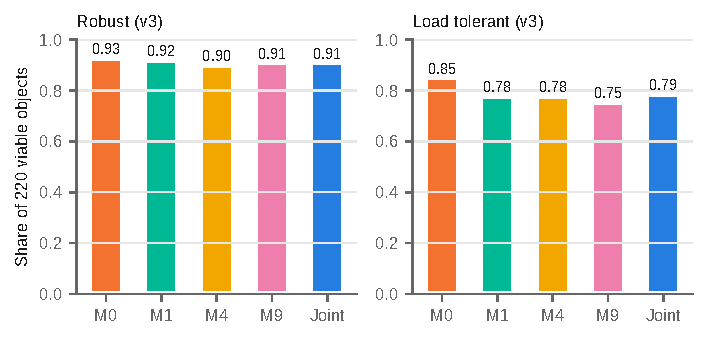
\includegraphics[width=\textwidth]{figures/fig_conf_rates.pdf}
\caption{EGAD primary set: share of first viable grasps that are robust and load tolerant (v3, torsion 0.005~m) for every method.}
\end{figure}

\section{Execution record}
The confirmation ran in a cloud container that restarted once during the physics stage (after 63 of the viable objects). Stages write one file per object only when the object is complete, so the run was resumed with the same frozen code and inputs; objects in progress at the restart were simulated again from scratch. No object was re-run because of its outcome. The frozen code hashes were checked before the analysis.

\end{document}
